\documentclass[12pt,a4paper]{article}

%% ---- Packages ----
\usepackage[utf8]{inputenc}
\usepackage[T1]{fontenc}
\usepackage{amsmath,amssymb,amsthm,mathtools}
\usepackage{hyperref}
\usepackage{cleveref}
\usepackage{graphicx}
\usepackage{geometry}
\usepackage{tikz-cd}
\usepackage{tikz}
\usetikzlibrary{decorations.pathmorphing,arrows.meta,positioning,calc,patterns,shapes.geometric}
\usepackage{enumitem}
\usepackage{xcolor}
\usepackage{fancyhdr}
\usepackage{everypage}
\usepackage{abstract}
\usepackage{setspace}
\usepackage{booktabs}
\usepackage{float}
\usepackage{caption}

\geometry{margin=1in}

%% ---- GrokRxiv DOI sidebar (official template) ----
\definecolor{grokgray}{RGB}{110,110,110}

\AddEverypageHook{%
  \ifnum\value{page}=1
    \begin{tikzpicture}[remember picture, overlay]
      \node[
        rotate=90,
        anchor=south,
        font=\Large\sffamily\bfseries\color{grokgray},
        inner sep=0pt
      ] at ([xshift=38pt, yshift=0.52\paperheight]current page.south west)
      {GrokRxiv:2026.02.measurement-problem-yoneda\quad
       [\,quant-ph\,]\quad
       17 Feb 2026};
    \end{tikzpicture}
  \fi
}

%% ---- Theorem environments ----
\theoremstyle{plain}
\newtheorem{theorem}{Theorem}[section]
\newtheorem{proposition}[theorem]{Proposition}
\newtheorem{lemma}[theorem]{Lemma}
\newtheorem{corollary}[theorem]{Corollary}
\newtheorem{conjecture}[theorem]{Conjecture}
\theoremstyle{definition}
\newtheorem{definition}[theorem]{Definition}
\newtheorem{example}[theorem]{Example}
\newtheorem{axiom}[theorem]{Axiom}
\newtheorem{remark}[theorem]{Remark}
\newtheorem{observation}[theorem]{Observation}

%% ---- Custom commands ----
\newcommand{\catC}{\mathcal{C}}
\newcommand{\catD}{\mathcal{D}}
\newcommand{\catMeas}{\mathbf{Meas}}
\newcommand{\catHilb}{\mathbf{Hilb}}
\newcommand{\catFdHilb}{\mathbf{FdHilb}}
\newcommand{\catSet}{\mathbf{Set}}
\newcommand{\catTop}{\mathbf{Top}}
\newcommand{\catCstar}{C^{*}\text{-}\mathbf{Alg}}
\newcommand{\catvNAlg}{\mathbf{vNAlg}}
\newcommand{\catCPTP}{\mathbf{CPTP}}
\newcommand{\Sys}{\mathcal{S}}
\newcommand{\Env}{\mathcal{E}}
\newcommand{\R}{\mathcal{R}}
\newcommand{\Hilb}{\mathcal{H}}
\newcommand{\Alg}{\mathcal{A}}
\newcommand{\Obs}{\mathcal{O}}
\newcommand{\State}{\mathcal{S}}
\newcommand{\Pre}{\mathcal{P}}
\newcommand{\Emer}{\mathcal{E}}
\newcommand{\Hom}{\mathrm{Hom}}
\newcommand{\id}{\mathrm{id}}
\newcommand{\op}{\mathrm{op}}
\newcommand{\Lan}{\mathrm{Lan}}
\newcommand{\Ran}{\mathrm{Ran}}
\newcommand{\coker}{\mathrm{coker}}
\newcommand{\im}{\mathrm{im}}
\newcommand{\Tr}{\mathrm{Tr}}
\newcommand{\rank}{\mathrm{rank}}
\newcommand{\Ob}{\mathrm{Ob}}
\newcommand{\Mor}{\mathrm{Mor}}
\newcommand{\Nat}{\mathrm{Nat}}
\newcommand{\PSh}{\mathrm{PSh}}
\newcommand{\yo}{\mathsf{y}}
\newcommand{\ket}[1]{|#1\rangle}
\newcommand{\bra}[1]{\langle#1|}
\newcommand{\braket}[2]{\langle#1|#2\rangle}
\newcommand{\ketbra}[2]{|#1\rangle\langle#2|}
\newcommand{\expect}[1]{\langle#1\rangle}

\hypersetup{
  colorlinks=true,
  linkcolor=blue!70!black,
  citecolor=green!50!black,
  urlcolor=blue!60!black,
  pdftitle={The Measurement Problem as a Yoneda Obstruction},
  pdfauthor={Matthew Long, The YonedaAI Collaboration}
}

%% ---- Page style ----
\pagestyle{fancy}
\fancyhf{}
\fancyhead[L]{\small\textit{The Measurement Problem as a Yoneda Obstruction}}
\fancyhead[R]{\small\thepage}
\renewcommand{\headrulewidth}{0.4pt}

%% ---- Title ----
\title{%
  \vspace{-1cm}
  \textbf{The Measurement Problem as a Yoneda Obstruction:}\\[6pt]
  \large Category-Theoretic Foundations for the\\
  Quantum-to-Classical Transition and Observer-Relative Collapse
}

\author{
  \textbf{Matthew Long}\\[4pt]
  The YonedaAI Collaboration\\
  YonedaAI Research Collective\\
  Chicago, IL\\[2pt]
  \texttt{matthew@yonedaai.com} $\cdot$ \url{https://yonedaai.com}
}

\date{February 2026}

\begin{document}

\maketitle

% ============================================================
% ABSTRACT
% ============================================================
\begin{abstract}
\noindent
We present a rigorous category-theoretic reformulation of the quantum measurement problem in which the apparent ``collapse of the wave function'' is identified as a structural obstruction arising from the Yoneda lemma applied to embedded observers in quantum measurement categories. The \emph{Yoneda Constraint on Observer Knowledge}---that an embedded observer $\Sys$ accesses reality $\R$ only through the representable presheaf $\Hom_{\catMeas}((\Sys, \R|_\Sys), -)$---implies that the measurement problem is not a dynamical puzzle requiring a new physical mechanism but a \emph{categorical inevitability}: the non-existence of a natural isomorphism between the observer's local presheaf and the global state functor. We develop this perspective through five main results. First, we prove that the measurement transition (from superposition to definite outcome) corresponds precisely to the failure of the Yoneda embedding to extend from a quantum subcategory to a classical one (Theorem~\ref{thm:measurement-obstruction}). Second, we show that decoherence provides a \emph{Kan extension} that is the optimal but necessarily lossy approximation bridging this gap (Theorem~\ref{thm:decoherence-kan}). Third, we establish that the Born rule emerges as the unique natural transformation compatible with the Yoneda structure (Theorem~\ref{thm:born-naturality}). Fourth, we prove that Wigner's friend scenarios manifest as coherence failures in 2-categorical extensions of the measurement category (Theorem~\ref{thm:wigner-coherence}). Fifth, we demonstrate that the Measurement Boundary Problem of emergent spacetime physics---the circularity of using spacetime-embedded detectors to probe the pre-geometric substrate---is a higher-order instance of the same Yoneda obstruction (Theorem~\ref{thm:mbp-yoneda}). Accompanying Haskell code provides executable models of these categorical structures.

\vspace{8pt}
\noindent\textbf{Keywords:} measurement problem, Yoneda lemma, category theory, quantum foundations, decoherence, Born rule, Wigner's friend, Kan extensions, embedded observers, representable presheaves, emergent spacetime
\end{abstract}

\tableofcontents
\newpage

% ============================================================
% 1. INTRODUCTION
% ============================================================
\section{Introduction}\label{sec:intro}

The measurement problem remains the central conceptual puzzle of quantum mechanics. In its sharpest form, it asks: how does the deterministic, unitary, linear evolution of the quantum state give rise to the apparently stochastic, irreversible, nonlinear ``collapse'' that produces definite measurement outcomes? After nearly a century of debate, the competing answers---Copenhagen interpretation, many-worlds, decoherence, objective collapse, relational quantum mechanics, QBism---continue to proliferate without consensus \cite{wheeler1983,zurek2003,schlosshauer2007}.

In this paper, we argue that the measurement problem admits a precise and illuminating reformulation in the language of category theory, specifically through the machinery of the Yoneda lemma, representable presheaves, and Kan extensions. Our central thesis is:

\begin{quote}
\emph{The measurement problem is not a dynamical puzzle requiring a new physical mechanism. It is a categorical obstruction: the structural impossibility of extending the Yoneda-representable knowledge of an embedded quantum observer to encompass the global unitary evolution of the total system.}
\end{quote}

This perspective builds on and synthesizes three lines of prior work within the YonedaAI research program:
\begin{enumerate}[label=(\roman*)]
  \item The \emph{Yoneda Constraint on Observer Knowledge} \cite{long2026yoneda}, which establishes that an embedded observer's epistemic access to reality is completely determined by its representable presheaf in the measurement category, and that this presheaf is generically incomplete when the observer is a proper subsystem.
  \item The \emph{Embedded Observer Constraint} \cite{long2026eoc}, which formalizes the information-theoretic, topological, and self-referential limitations on subsystem-internal description.
  \item The \emph{Measurement Boundary Problem} in emergent spacetime physics \cite{long2026mbp}, which identifies a circularity in using spacetime-based apparatus to probe the pre-geometric substrate from which spacetime arises.
\end{enumerate}

The present paper demonstrates that the standard quantum measurement problem and the Measurement Boundary Problem are both instances of a single categorical phenomenon: the failure of a Yoneda extension across an emergence boundary. This unification provides structural clarity and suggests that the resolution of the measurement problem lies not in choosing among interpretations but in understanding the categorical constraints that any interpretation must satisfy.

\subsection{Overview of Results}

Our main contributions are the following:

\textbf{The Measurement Obstruction Theorem} (\S\ref{sec:obstruction}, Theorem~\ref{thm:measurement-obstruction}): We prove that the measurement transition---from quantum superposition to definite classical outcome---corresponds to the non-existence of a fully faithful functor from the classical outcome category to the quantum state category that is simultaneously compatible with the Yoneda embedding and the Born rule. The obstruction is measured by a cohomological invariant that we explicitly construct.

\textbf{Decoherence as Kan Extension} (\S\ref{sec:decoherence}, Theorem~\ref{thm:decoherence-kan}): We show that the decoherence program, which explains the emergence of classicality through environmental entanglement, is precisely a left Kan extension of the observer's local description functor along the inclusion of the accessible subcategory. This Kan extension is the best possible approximation to the global description but is necessarily lossy---the extension deficit is quantified by the decoherence-induced entropy.

\textbf{The Born Rule as Natural Transformation} (\S\ref{sec:born}, Theorem~\ref{thm:born-naturality}): We prove that the Born rule $p_i = \Tr(\rho E_i)$ is the \emph{unique} natural transformation from the representable presheaf of an observer in $\catMeas_Q$ to the probability functor, subject to normalization and functoriality constraints. This provides a structural derivation of the Born rule from the Yoneda framework.

\textbf{Wigner's Friend as 2-Categorical Coherence Failure} (\S\ref{sec:wigner}, Theorem~\ref{thm:wigner-coherence}): We show that Wigner's friend scenarios---where two observers give conflicting accounts of a measurement---arise as failures of coherence conditions in the 2-category $\catMeas_2$, where 2-cells represent observer transformations. The paradox dissolves once one recognizes that different observers inhabit different representable presheaves with no obligation of mutual consistency.

\textbf{The Measurement Boundary Problem as Higher Yoneda Obstruction} (\S\ref{sec:mbp}, Theorem~\ref{thm:mbp-yoneda}): We demonstrate that the Measurement Boundary Problem of emergent spacetime---the circularity of spacetime-based measurements probing the pre-geometric substrate---is a higher-order instance of the measurement obstruction, operating at the level of emergence functors between measurement categories rather than within a single category.

\subsection{Relation to Interpretations of Quantum Mechanics}

Our framework is not another interpretation of quantum mechanics. Rather, it identifies categorical constraints that any adequate interpretation must satisfy. Nevertheless, it has differential implications for existing interpretations:

\begin{itemize}[leftmargin=2em]
  \item \textbf{Copenhagen}: The Yoneda framework provides a mathematical justification for the Copenhagen distinction between ``system'' and ``apparatus,'' identifying it as the distinction between the representable presheaf of the observer and the global state functor.
  \item \textbf{Many-worlds}: The many-worlds interpretation corresponds to working with the full category $\catMeas_Q$ rather than any single representable presheaf. The ``branching'' is the proliferation of non-isomorphic objects in $\catMeas_Q$ under decoherence.
  \item \textbf{Relational QM}: Rovelli's relational quantum mechanics \cite{rovelli1996} is the closest philosophical precursor. The Yoneda Constraint formalizes and extends the relational insight: quantum states are representable presheaves, and different observers have different (and generally incompatible) presheaves.
  \item \textbf{QBism}: The QBist emphasis on the agent's epistemic state aligns with our presheaf-theoretic formulation, but the Yoneda framework grounds the agent's perspective in mathematical structure rather than subjective probability.
\end{itemize}


% ============================================================
% 2. CATEGORICAL PREREQUISITES
% ============================================================
\section{Categorical Prerequisites}\label{sec:background}

We briefly recall the categorical machinery used throughout. The reader familiar with category theory may skip to \S\ref{sec:measurement-category}.

\subsection{The Yoneda Lemma}

Let $\catC$ be a locally small category. For each object $A \in \catC$, the \emph{representable presheaf} is the functor $\yo_A = \Hom_\catC(A, -): \catC \to \catSet$.

\begin{theorem}[Yoneda Lemma \cite{maclane1998}]\label{thm:yoneda-recall}
For any functor $F: \catC \to \catSet$ and object $A \in \catC$, there is a bijection
\[
\Nat(\Hom_\catC(A, -), F) \cong F(A)
\]
natural in both $A$ and $F$.
\end{theorem}

The \emph{Yoneda embedding} $\yo: \catC \hookrightarrow [\catC^{\op}, \catSet]$ is full and faithful: an object is completely determined (up to isomorphism) by the totality of morphisms into (or out of) it.

\subsection{Kan Extensions}

Given functors $K: \catC \to \catD$ and $F: \catC \to \Emer$, the \emph{left Kan extension} $\Lan_K F: \catD \to \Emer$ is the universal functor satisfying the appropriate universal property. When it exists pointwise:
\[
(\Lan_K F)(d) = \mathrm{colim}_{(c, K(c) \to d) \in (K \downarrow d)} F(c).
\]
The right Kan extension is defined dually via limits.

\subsection{2-Categories}

A \emph{2-category} $\catC$ has objects (0-cells), morphisms (1-cells), and 2-morphisms (2-cells) between parallel 1-cells. Composition is defined both vertically (composing 2-cells at the same 1-cell) and horizontally (composing along 1-cells), subject to the interchange law.

\subsection{Enriched Categories}

A $\mathcal{V}$-enriched category replaces hom-sets with objects of a monoidal category $(\mathcal{V}, \otimes, I)$. For quantum mechanics, the relevant enrichment is over Hilbert spaces or $C^*$-algebras.


% ============================================================
% 3. THE MEASUREMENT CATEGORY
% ============================================================
\section{The Quantum Measurement Category}\label{sec:measurement-category}

\subsection{Definition and Structure}

\begin{definition}[Quantum Measurement Category]\label{def:qmeas}
The \emph{quantum measurement category} $\catMeas_Q$ is a category whose:
\begin{enumerate}[label=(\roman*),itemsep=4pt]
\item \textbf{Objects} are triples $(\Sys, \Hilb_\Sys, \rho_\Sys)$ where $\Sys$ is a physical subsystem, $\Hilb_\Sys$ is its Hilbert space, and $\rho_\Sys \in \mathcal{B}(\Hilb_\Sys)$ is a density operator representing the observer's state (or the state accessible to the observer).
\item \textbf{Morphisms} $f: (\Sys_1, \Hilb_1, \rho_1) \to (\Sys_2, \Hilb_2, \rho_2)$ are completely positive trace-preserving (CPTP) maps $\Phi_f: \mathcal{B}(\Hilb_1) \to \mathcal{B}(\Hilb_2)$ such that $\Phi_f(\rho_1) = \rho_2$.
\item \textbf{Composition} is the composition of CPTP maps.
\item \textbf{Identity} morphisms are the identity channels.
\end{enumerate}
\end{definition}

\begin{definition}[Classical Outcome Category]\label{def:classical-cat}
The \emph{classical outcome category} $\catMeas_C$ is the full subcategory of $\catMeas_Q$ whose objects $(\Sys, \Hilb_\Sys, \rho_\Sys)$ satisfy:
\begin{enumerate}[label=(\roman*)]
\item $\rho_\Sys$ is diagonal in a preferred basis (the pointer basis);
\item morphisms between objects in $\catMeas_C$ preserve diagonality.
\end{enumerate}
\end{definition}

The inclusion functor $\iota: \catMeas_C \hookrightarrow \catMeas_Q$ embeds classical outcomes into the quantum category. The measurement problem, in categorical language, concerns the relationship between $\catMeas_Q$ and $\catMeas_C$.

\subsection{The Embedded Observer}

\begin{definition}[Embedded Quantum Observer]\label{def:embedded-observer}
An \emph{embedded quantum observer} is an object $(\Sys, \Hilb_\Sys, \rho_\Sys) \in \catMeas_Q$ such that $\Sys$ is a proper subsystem of a total system $\R$:
\[
\Hilb_\R = \Hilb_\Sys \otimes \Hilb_\Env, \qquad \rho_\Sys = \Tr_\Env(\rho_\R).
\]
The environment $\Env$ comprises all degrees of freedom not directly accessible to $\Sys$.
\end{definition}

\begin{proposition}[Yoneda Constraint for Quantum Observers]\label{prop:yoneda-constraint-q}
The embedded quantum observer $(\Sys, \Hilb_\Sys, \rho_\Sys)$ knows the total system $\R$ only through the representable presheaf
\[
\yo_{(\Sys, \Hilb_\Sys, \rho_\Sys)} = \Hom_{\catMeas_Q}((\Sys, \Hilb_\Sys, \rho_\Sys), -).
\]
This presheaf determines $(\Sys, \Hilb_\Sys, \rho_\Sys)$ up to isomorphism (by the Yoneda lemma) but does not determine the global state $\rho_\R$ or the decomposition $\Hilb_\R = \Hilb_\Sys \otimes \Hilb_\Env$.
\end{proposition}

\begin{proof}
The Yoneda embedding is full and faithful, so $\yo_{(\Sys, \Hilb_\Sys, \rho_\Sys)}$ captures all categorical information about the observer's object. However, this object carries only $\rho_\Sys = \Tr_\Env(\rho_\R)$, which is informationally deficient relative to $\rho_\R$ whenever $\rho_\R$ is entangled across the $\Sys$--$\Env$ partition (i.e., whenever $S(\rho_\Sys) > 0$).
\end{proof}

\subsection{The State Functor and the Description Functor}

\begin{definition}[Global State Functor]\label{def:state-functor}
The \emph{global state functor} $\mathfrak{G}: \catMeas_Q \to \catSet$ assigns to each object $(\Sys, \Hilb_\Sys, \rho_\Sys)$ the set of all global pure states $\ket{\Psi} \in \Hilb_\R$ compatible with $\rho_\Sys$:
\[
\mathfrak{G}(\Sys, \Hilb_\Sys, \rho_\Sys) = \{ \ket{\Psi} \in \Hilb_\R : \Tr_\Env(\ketbra{\Psi}{\Psi}) = \rho_\Sys \}.
\]
\end{definition}

\begin{definition}[Local Description Functor]\label{def:local-functor}
The \emph{local description functor} $\mathfrak{L}: \catMeas_Q \to \catSet$ assigns to each object the set of measurement outcomes accessible to $\Sys$:
\[
\mathfrak{L}(\Sys, \Hilb_\Sys, \rho_\Sys) = \{ (E_i, p_i) : \{E_i\} \text{ is a POVM on } \Hilb_\Sys, \; p_i = \Tr(\rho_\Sys E_i) \}.
\]
\end{definition}

The measurement problem is the question of whether there exists a natural transformation $\eta: \mathfrak{L} \Rightarrow \mathfrak{G}$ that ``lifts'' local measurement data to global state determination.

\begin{proposition}[Non-Existence of Lifting]\label{prop:no-lifting}
For any embedded observer $\Sys \subsetneq \R$ with entangled $\rho_\R$, there is no natural isomorphism $\eta: \mathfrak{L} \Rightarrow \mathfrak{G}$. The global state functor is not representable by the observer's local data.
\end{proposition}

\begin{proof}
By the non-uniqueness of purification: for any mixed $\rho_\Sys$, the fiber $\mathfrak{G}(\Sys, \Hilb_\Sys, \rho_\Sys)$ contains infinitely many distinct global states (related by unitaries on $\Hilb_\Env$). No local POVM data can discriminate among these. The cardinality mismatch between $\mathfrak{L}$ and $\mathfrak{G}$ prevents any natural isomorphism.
\end{proof}


% ============================================================
% 4. THE MEASUREMENT OBSTRUCTION
% ============================================================
\section{The Measurement Obstruction Theorem}\label{sec:obstruction}

We now state and prove the central result: the measurement problem is a Yoneda obstruction.

\subsection{Formulation}

Consider the diagram of categories and functors:
\[
\begin{tikzcd}[column sep=large, row sep=large]
\catMeas_C \arrow[r, hook, "\iota"] \arrow[d, "\yo_C"'] & \catMeas_Q \arrow[d, "\yo_Q"] \\
\PSh(\catMeas_C) \arrow[r, dashed, "\Phi?"] & \PSh(\catMeas_Q)
\end{tikzcd}
\]
Here $\yo_C$ and $\yo_Q$ are the Yoneda embeddings of the classical and quantum measurement categories, and $\Phi$ is a hypothetical functor making the diagram commute. The measurement problem asks: under what conditions does $\Phi$ exist?

\subsection{The Obstruction}

\begin{theorem}[Measurement Obstruction]\label{thm:measurement-obstruction}
Let $\iota: \catMeas_C \hookrightarrow \catMeas_Q$ be the inclusion of the classical outcome category into the quantum measurement category. There is no functor $\Phi: \PSh(\catMeas_C) \to \PSh(\catMeas_Q)$ such that:
\begin{enumerate}[label=(\alph*)]
\item $\Phi$ makes the above diagram commute up to natural isomorphism;
\item $\Phi$ preserves the probability structure (i.e., is compatible with the Born rule);
\item $\Phi$ is fully faithful.
\end{enumerate}
The obstruction is classified by the \emph{measurement cohomology class} $[\omega_M] \in H^2(\catMeas_C; \mathcal{U}(\Hilb_\Env))$, where $\mathcal{U}(\Hilb_\Env)$ is the unitary group of the environment.
\end{theorem}

\begin{proof}
We proceed by contradiction. Suppose $\Phi$ exists satisfying (a)--(c).

\textbf{Step 1: Presheaf structure.} By condition (a), for each classical outcome object $c = (\Sys, \Hilb_\Sys, \rho_c) \in \catMeas_C$ (with $\rho_c$ diagonal in the pointer basis), we have
\[
\Phi(\yo_C(c)) \cong \yo_Q(\iota(c)).
\]
This means the presheaf of the classical outcome, when embedded in the quantum category, is representable.

\textbf{Step 2: Born rule compatibility.} Consider a quantum state $\rho_\Sys = \sum_i p_i \ketbra{a_i}{a_i}$ (in the pointer basis). The Born rule assigns probabilities $p_i = \Tr(\rho_\Sys \ketbra{a_i}{a_i})$ to each classical outcome. By condition (b), $\Phi$ must respect these probabilities:
\[
\Phi(\yo_C(c_i)) \cong \yo_Q(\iota(c_i)) \quad \text{with weight } p_i.
\]

\textbf{Step 3: Faithfulness obstruction.} By condition (c), $\Phi$ is fully faithful. This means it preserves and reflects all morphism structure. However, in $\PSh(\catMeas_Q)$, the pre-measurement quantum state $\rho_\Sys$ (which is a superposition in a complementary basis) defines morphisms that have no counterpart in $\PSh(\catMeas_C)$---specifically, the off-diagonal coherences $\rho_{ij} = \langle a_i | \rho_\Sys | a_j \rangle$ for $i \neq j$ generate morphisms in $\catMeas_Q$ that are annihilated by the inclusion $\iota$. A fully faithful $\Phi$ cannot both preserve these morphisms and map into the image of the classical embedding.

\textbf{Step 4: Cohomological classification.} We construct the obstruction cocycle explicitly. Consider the nerve of the cover $\{U_i\}$ of $\catMeas_C$ by neighborhoods of classical outcomes $c_i$. For each pair $(c_i, c_j)$, the overlap $U_i \cap U_j$ in $\catMeas_Q$ consists of quantum states that can be reached from both classical outcomes via CPTP maps. The purification theorem provides, for each $c_i$, a purification $\ket{\Psi_i} \in \Hilb_\Sys \otimes \Hilb_\Env$ with $\Tr_\Env(\ketbra{\Psi_i}{\Psi_i}) = \rho_{c_i}$. The transition function on the overlap is the unitary $U_{ij} \in \mathcal{U}(\Hilb_\Env)$ satisfying $\ket{\Psi_j} = (\mathbb{1}_\Sys \otimes U_{ij})\ket{\Psi_i}$.

For a triple $(c_i, c_j, c_k)$, the cocycle condition requires $U_{ij} U_{jk} U_{ki} = \mathbb{1}$. The 2-cocycle is
\[
\omega_M(c_i, c_j, c_k) = U_{ij} U_{jk} U_{ki} \in \mathcal{U}(\Hilb_\Env).
\]
The class $[\omega_M] \in H^2(\catMeas_C; \mathcal{U}(\Hilb_\Env))$ is independent of the choice of purifications (different purification choices change the cocycle by a coboundary). The obstruction $[\omega_M]$ vanishes if and only if there exists a consistent global choice of purifications---equivalently, a fully faithful $\Phi$.

For generic entangled states, $[\omega_M] \neq 0$ because the purification degeneracy (the $\mathcal{U}(\Hilb_\Env)$-freedom in choosing environmental states) cannot be consistently resolved across all measurement contexts. A computable scalar witness for non-triviality is the off-diagonal $l_2$-coherence $C(\rho) = \sum_{i \neq j} |\rho_{ij}|^2$: when $C(\rho) > 0$, the cocycle is non-trivial.
\end{proof}

\begin{corollary}[Interpretation-Independence of the Obstruction]\label{cor:interpretation}
The measurement obstruction $[\omega_M]$ is independent of the choice of interpretation of quantum mechanics. It is a structural feature of the relationship between $\catMeas_C$ and $\catMeas_Q$, not an artifact of any particular interpretive framework.
\end{corollary}

\subsection{Physical Significance}

The Measurement Obstruction Theorem tells us that the measurement problem is not about missing physics but about categorical structure. The quantum and classical descriptions live in different presheaf categories, and no fully faithful, probability-preserving functor connects them. Every interpretation of quantum mechanics is, from this perspective, a \emph{strategy for coping with this obstruction}:

\begin{itemize}[leftmargin=2em]
\item \textbf{Copenhagen}: Accepts the obstruction and draws a pragmatic boundary between $\catMeas_C$ and $\catMeas_Q$.
\item \textbf{Many-worlds}: Works entirely in $\PSh(\catMeas_Q)$, avoiding the need for $\Phi$.
\item \textbf{Decoherence}: Constructs an approximate $\Phi$ via Kan extension (see \S\ref{sec:decoherence}).
\item \textbf{Objective collapse}: Modifies the dynamics of $\catMeas_Q$ to make the obstruction vanish.
\item \textbf{Relational QM}: Relativizes $\Phi$ to each observer's presheaf.
\end{itemize}


% ============================================================
% 5. DECOHERENCE AS KAN EXTENSION
% ============================================================
\section{Decoherence as Kan Extension}\label{sec:decoherence}

The decoherence program \cite{zurek2003,schlosshauer2007} provides the most widely accepted partial resolution of the measurement problem. We now show that decoherence is precisely a left Kan extension that provides the optimal (but lossy) bridge between the quantum and classical measurement categories.

\subsection{The Decoherence Functor}

\begin{definition}[Decoherence Functor]\label{def:decoherence}
The \emph{decoherence functor} $\mathcal{D}: \catMeas_Q \to \catMeas_Q$ is defined on objects by
\[
\mathcal{D}(\Sys, \Hilb_\Sys, \rho_\Sys) = (\Sys, \Hilb_\Sys, \Delta(\rho_\Sys))
\]
where $\Delta(\rho_\Sys) = \sum_i \langle a_i | \rho_\Sys | a_i \rangle \ketbra{a_i}{a_i}$ is the dephasing map in the pointer basis $\{\ket{a_i}\}$, and on morphisms by the induced CPTP maps.
\end{definition}

The decoherence functor annihilates off-diagonal coherences, projecting quantum states onto classical probability distributions over pointer states. Its image lies in $\catMeas_C$.

\begin{proposition}[Decoherence as Projection]\label{prop:decoherence-projection}
The decoherence functor $\mathcal{D}$ satisfies:
\begin{enumerate}[label=(\alph*)]
\item $\mathcal{D} \circ \mathcal{D} \cong \mathcal{D}$ (idempotent);
\item $\im(\mathcal{D}) \cong \catMeas_C$ (image is the classical subcategory);
\item $\mathcal{D} \circ \iota \cong \id_{\catMeas_C}$ (left inverse of the inclusion on objects).
\end{enumerate}
\end{proposition}

\subsection{The Kan Extension Structure}

\begin{theorem}[Decoherence as Left Kan Extension]\label{thm:decoherence-kan}
The decoherence functor $\mathcal{D}$ is (isomorphic to) the left Kan extension of the identity functor on $\catMeas_C$ along the inclusion $\iota: \catMeas_C \hookrightarrow \catMeas_Q$:
\[
\mathcal{D} \cong \Lan_\iota(\id_{\catMeas_C}).
\]
That is, decoherence is the ``best approximation'' to the classical identity, extended from the classical subcategory to the full quantum category. The approximation is optimal in the sense of the universal property of Kan extensions: for any other functor $G: \catMeas_Q \to \catMeas_C$ with $G \circ \iota \cong \id_{\catMeas_C}$, there exists a unique natural transformation $\mathcal{D} \Rightarrow G$.
\end{theorem}

\begin{proof}
We verify the universal property. For any functor $G: \catMeas_Q \to \catMeas_C$ with $G \circ \iota \cong \id_{\catMeas_C}$, we must construct a natural transformation $\alpha: \mathcal{D} \Rightarrow G$.

For each object $q = (\Sys, \Hilb_\Sys, \rho_\Sys) \in \catMeas_Q$, the pointwise formula gives:
\[
(\Lan_\iota \id)(q) = \mathrm{colim}_{(c, \iota(c) \to q) \in (\iota \downarrow q)} c.
\]
The category $(\iota \downarrow q)$ has objects $(c, f)$ where $c \in \catMeas_C$ and $f: \iota(c) \to q$ is a CPTP map sending the classical state to $\rho_\Sys$. The colimit over these objects is the ``best classical state reachable from $q$,'' which is precisely $\Delta(\rho_\Sys)$---the diagonal part of $\rho_\Sys$ in the pointer basis.

The natural transformation $\alpha: \mathcal{D} \Rightarrow G$ is constructed by the universal property: since $G$ also sends $q$ to a classical state compatible with $\rho_\Sys$, and $\mathcal{D}(q) = \Delta(\rho_\Sys)$ is the universal such state, there is a unique map $\alpha_q: \Delta(\rho_\Sys) \to G(q)$ in $\catMeas_C$.
\end{proof}

\subsection{The Extension Deficit}

\begin{definition}[Decoherence Deficit]\label{def:deficit}
The \emph{decoherence deficit} of the Kan extension is the natural transformation
\[
\delta: \yo_Q \Rightarrow \yo_Q \circ \mathcal{D}
\]
whose kernel measures the quantum coherences lost in the decoherence process. The \emph{deficit entropy} is
\[
S_\delta(\rho_\Sys) = S(\Delta(\rho_\Sys)) - S(\rho_\Sys) \geq 0,
\]
where $S$ denotes von Neumann entropy. The deficit entropy vanishes if and only if $\rho_\Sys$ is already classical (diagonal in the pointer basis).
\end{definition}

\begin{proposition}[Information Loss in the Kan Extension]\label{prop:info-loss}
The decoherence deficit quantifies the information about the global state $\rho_\R$ that is irretrievably lost when the observer's description is extended from the quantum to the classical category via the Kan extension. Specifically:
\[
I_{\text{lost}} = S(\Delta(\rho_\Sys)) - S(\rho_\Sys) = -\sum_i p_i \log p_i - S(\rho_\Sys),
\]
where $p_i = \langle a_i | \rho_\Sys | a_i \rangle$ and $S(\rho_\Sys)$ is the von Neumann entropy of the full quantum state.
\end{proposition}

\begin{corollary}[Decoherence Does Not Solve the Measurement Problem]\label{cor:decoherence-incomplete}
Since the Kan extension is necessarily lossy (the deficit entropy is generically positive for quantum states), decoherence alone does not provide a natural isomorphism $\Phi: \PSh(\catMeas_C) \to \PSh(\catMeas_Q)$. The measurement obstruction (Theorem~\ref{thm:measurement-obstruction}) persists even after decoherence.
\end{corollary}

This corollary aligns with the well-known criticism that decoherence explains the \emph{appearance} of collapse (the suppression of interference) but does not explain why a \emph{specific} outcome occurs. In our framework, this limitation is a consequence of the universal property of Kan extensions: they provide the best approximation, not an exact reconstruction.

\begin{remark}[The Right Kan Extension and Conservative Extrapolation]\label{rem:right-kan}
The right Kan extension $\Ran_\iota(\id_{\catMeas_C})$ provides a dual, ``conservative'' approximation. While the left Kan extension (decoherence) projects quantum states onto their diagonal components---the most ``optimistic'' classical approximation---the right Kan extension yields the maximally mixed state over the support of the diagonal, representing the most ``pessimistic'' classical description compatible with the quantum data. The true description is bracketed:
\[
\Lan_\iota(\id) \Rightarrow \mathfrak{R} \Rightarrow \Ran_\iota(\id).
\]
Physically, the left Kan extension corresponds to the environment ``selecting'' a pointer basis (decoherence), while the right Kan extension corresponds to the observer making no assumption about which outcome has occurred. The width of this bracket---the difference between the two Kan extensions---measures the fundamental ambiguity in the quantum-to-classical transition that cannot be resolved by categorical considerations alone.
\end{remark}


% ============================================================
% 6. THE BORN RULE AS NATURAL TRANSFORMATION
% ============================================================
\section{The Born Rule as Natural Transformation}\label{sec:born}

\subsection{The Probability Functor}

\begin{definition}[Probability Functor]\label{def:prob-functor}
The \emph{probability functor} $\mathcal{P}: \catMeas_Q \to [0,1]\text{-}\catSet$ assigns to each object $(\Sys, \Hilb_\Sys, \rho_\Sys)$ the set of probability distributions over measurement outcomes:
\[
\mathcal{P}(\Sys, \Hilb_\Sys, \rho_\Sys) = \left\{ (p_1, \ldots, p_n) : p_i \geq 0, \sum_i p_i = 1, \; n = \dim \Hilb_\Sys \right\}.
\]
Morphisms (CPTP maps) act by the induced stochastic maps on probability distributions.
\end{definition}

\subsection{Derivation of the Born Rule}

\begin{theorem}[Born Rule as Unique Natural Transformation]\label{thm:born-naturality}
The Born rule defines the unique natural transformation $\beta: \yo_{(\Sys, \Hilb_\Sys, \rho_\Sys)} \Rightarrow \mathcal{P}$ satisfying:
\begin{enumerate}[label=(\roman*)]
\item \textbf{Normalization}: For each measurement context (POVM $\{E_i\}$), the probabilities sum to 1.
\item \textbf{Functoriality}: The probabilities are consistent under CPTP maps (measurement refinements).
\item \textbf{State determination}: The map $\rho_\Sys \mapsto \{\Tr(\rho_\Sys E_i)\}_i$ determines $\rho_\Sys$ uniquely (quantum state tomography).
\end{enumerate}
The uniqueness follows from the Yoneda lemma: by Theorem~\ref{thm:yoneda-recall}, natural transformations from the representable presheaf to any functor $F$ are in bijection with $F(A)$, and the normalization and functoriality constraints single out the Born rule map $p_i = \Tr(\rho_\Sys E_i)$.
\end{theorem}

\begin{proof}
By the Yoneda lemma,
\[
\Nat(\yo_{(\Sys, \Hilb_\Sys, \rho_\Sys)}, \mathcal{P}) \cong \mathcal{P}(\Sys, \Hilb_\Sys, \rho_\Sys).
\]
An element of $\mathcal{P}(\Sys, \Hilb_\Sys, \rho_\Sys)$ is a probability distribution over measurement outcomes. The element corresponding to a POVM $\{E_i\}$ is uniquely determined by the requirements:
\begin{enumerate}[label=(\alph*)]
\item $p_i \geq 0$ for all $i$ (positivity of CPTP maps);
\item $\sum_i p_i = 1$ (trace preservation);
\item $p_i$ is linear in $\rho_\Sys$ (linearity of the trace);
\item $p_i$ is linear in $E_i$ (linearity of the trace);
\item For $E_i = \ketbra{\psi}{\psi}$ and $\rho_\Sys = \ketbra{\phi}{\phi}$, we need $p_i = |\braket{\psi}{\phi}|^2$ (standard overlap for pure states, by Gleason's theorem for $\dim \Hilb_\Sys \geq 3$).
\end{enumerate}
The unique linear functional satisfying (a)--(e) is $p_i = \Tr(\rho_\Sys E_i)$, which is the Born rule.

Naturality follows from the CPTP structure: for a morphism $f: (\Sys_1, \Hilb_1, \rho_1) \to (\Sys_2, \Hilb_2, \rho_2)$ with associated CPTP map $\Phi_f$, the Born probabilities transform as $p_i^{(2)} = \Tr(\Phi_f(\rho_1) E_i^{(2)}) = \Tr(\rho_1 \Phi_f^*(E_i^{(2)}))$, where $\Phi_f^*$ is the Heisenberg dual. This is precisely the functorial action of $\mathcal{P}$ on morphisms.
\end{proof}

\begin{corollary}[Born Rule from Yoneda + Gleason]\label{cor:born-gleason}
The Born rule is the unique probability assignment compatible with:
\begin{enumerate}[label=(\roman*)]
\item The Yoneda representation of the observer (relational knowledge);
\item Gleason's theorem (non-contextual probability on Hilbert space);
\item Functoriality of $\catMeas_Q$ (consistency under CPTP maps).
\end{enumerate}
\end{corollary}

\subsection{The Born Rule and the Measurement Obstruction}

The Born rule interacts with the measurement obstruction as follows:

\begin{proposition}[Born Rule as Partial Resolution]\label{prop:born-partial}
The Born rule provides a natural transformation $\beta: \yo \Rightarrow \mathcal{P}$ that partially resolves the measurement obstruction: it consistently assigns probabilities to classical outcomes, but it does not specify \emph{which} outcome occurs. The Born rule determines the statistical behavior of the Kan extension but not the individual realization.
\end{proposition}

This captures the well-known fact that quantum mechanics predicts probabilities but not individual outcomes. In our framework, this is not a deficiency of the theory but a structural consequence of the categorical relationship between $\catMeas_Q$ and $\catMeas_C$.


% ============================================================
% 7. WIGNER'S FRIEND AS 2-CATEGORICAL COHERENCE FAILURE
% ============================================================
\section{Wigner's Friend Scenarios}\label{sec:wigner}

The Wigner's friend thought experiment \cite{wigner1961} sharpens the measurement problem by introducing two observers who give conflicting accounts of a measurement. Recent extensions by Frauchiger and Renner \cite{frauchiger2018} and Brukner \cite{brukner2018} have generated renewed interest. We show that the Wigner's friend scenario is naturally analyzed as a coherence failure in the 2-category of measurements.

\subsection{The 2-Categorical Measurement Structure}

\begin{definition}[2-Categorical Measurement Category]\label{def:2meas}
The 2-category $\catMeas_2$ has:
\begin{enumerate}[label=(\roman*),itemsep=4pt]
\item \textbf{0-cells}: Objects of $\catMeas_Q$ (observer-state pairs $(\Sys, \Hilb_\Sys, \rho_\Sys)$).
\item \textbf{1-cells}: CPTP maps $\Phi: \mathcal{B}(\Hilb_1) \to \mathcal{B}(\Hilb_2)$ (measurements and state transformations).
\item \textbf{2-cells}: Given parallel 1-cells $\Phi, \Psi: (\Sys_1, \Hilb_1, \rho_1) \to (\Sys_2, \Hilb_2, \rho_2)$, a 2-cell $\alpha: \Phi \Rightarrow \Psi$ is a family of completely positive maps $\{\alpha_A\}_{A \in \mathcal{B}(\Hilb_2)}$ satisfying $\Psi(A) = \alpha_A(\Phi(A))$ for all $A$, subject to the constraint that $\alpha$ preserves the state: $\rho_2$ is invariant under $\alpha$. Physically, 2-cells represent basis changes or gauge transformations between measurement schemes that produce the same statistical predictions (same output state $\rho_2$).
\end{enumerate}
\end{definition}

\subsection{Wigner's Friend Setup}

Consider two observers:
\begin{itemize}[leftmargin=2em]
\item \textbf{Friend (F)}: Performs a measurement of spin along $z$ on a qubit $Q$ initially in state $\ket{+_x} = \frac{1}{\sqrt{2}}(\ket{\uparrow} + \ket{\downarrow})$.
\item \textbf{Wigner (W)}: Describes the Friend + Qubit system unitarily, as an entangled state $\frac{1}{\sqrt{2}}(\ket{\uparrow}\ket{F_\uparrow} + \ket{\downarrow}\ket{F_\downarrow})$.
\end{itemize}

In $\catMeas_2$, these correspond to two different objects:
\begin{align}
\text{Friend's object}: & \quad F = (\Sys_F, \Hilb_F, \rho_F) \quad \text{with } \rho_F = \ketbra{\uparrow}{\uparrow} \text{ or } \ketbra{\downarrow}{\downarrow} \\
\text{Wigner's object}: & \quad W = (\Sys_W, \Hilb_W, \rho_W) \quad \text{with } \rho_W = \ketbra{\Psi}{\Psi}
\end{align}
where $\ket{\Psi} = \frac{1}{\sqrt{2}}(\ket{\uparrow}\ket{F_\uparrow} + \ket{\downarrow}\ket{F_\downarrow})$.

\subsection{The Coherence Failure}

\begin{theorem}[Wigner's Friend as Coherence Failure]\label{thm:wigner-coherence}
In $\catMeas_2$, the Wigner's friend scenario generates a failure of the interchange law for 2-cells. Specifically, let:
\begin{itemize}
\item $\alpha: f \Rightarrow g$ be the 2-cell representing the Friend's measurement (collapsing the qubit state);
\item $\beta: h \Rightarrow k$ be the 2-cell representing Wigner's unitary description (entangling the Friend with the qubit).
\end{itemize}
Then the horizontal compositions $\beta \circ \alpha$ and $\alpha \circ \beta$ are not equal:
\[
\beta \circ_h \alpha \neq \alpha \circ_h \beta.
\]
The failure of the interchange law reflects the incompatibility of the two observers' descriptions.
\end{theorem}

\begin{proof}
The interchange law in a 2-category requires that for composable 2-cells,
\[
(\beta' \circ_v \beta) \circ_h (\alpha' \circ_v \alpha) = (\beta' \circ_h \alpha') \circ_v (\beta \circ_h \alpha).
\]
In the Wigner's friend scenario, the Friend's 2-cell $\alpha$ acts on the qubit subsystem (performing a projective measurement), while Wigner's 2-cell $\beta$ acts on the entire Friend+Qubit system (maintaining unitary evolution). These act on different objects in $\catMeas_2$, and their order of application matters: the Friend's measurement destroys coherences that Wigner's unitary evolution preserves.

Formally, let $\Phi_\alpha$ denote the CPTP map associated with the Friend's measurement and $U_\beta$ denote Wigner's unitary. Then:
\[
U_\beta \circ \Phi_\alpha(\rho_{QF}) \neq \Phi_\alpha \circ U_\beta(\rho_{QF})
\]
because $\Phi_\alpha$ is a non-unitary projection while $U_\beta$ preserves coherences. This non-commutativity at the level of 1-cells lifts to a coherence failure at the level of 2-cells.
\end{proof}

\begin{corollary}[Resolution via Perspectival Presheaves]\label{cor:wigner-resolution}
The Wigner's friend paradox dissolves in the Yoneda framework. The Friend and Wigner inhabit different representable presheaves:
\[
\yo_F = \Hom_{\catMeas_Q}(F, -), \qquad \yo_W = \Hom_{\catMeas_Q}(W, -).
\]
These are different presheaves on the same category, and there is no requirement that they be naturally isomorphic. Each observer's presheaf provides a complete and consistent account of reality from that observer's position. The ``paradox'' arises only from the assumption that there should be a single, observer-independent presheaf---an assumption that the Yoneda Constraint explicitly denies.
\end{corollary}

\subsection{Extended Wigner Scenarios}

The Frauchiger-Renner extension \cite{frauchiger2018} involves nested observers making inferences about each other's measurement outcomes. In our framework, this generates a tower of presheaves:
\[
\yo_{F_1}, \quad \yo_{F_2}, \quad \yo_{W_1}, \quad \yo_{W_2}, \quad \ldots
\]
The contradiction in the Frauchiger-Renner argument arises from treating these presheaves as mutually compatible (demanding a global section of their product presheaf). The Kochen-Specker theorem, in the form of the failure of global sections for the valuation presheaf \cite{abramsky2011}, guarantees that such a global section does not exist when the system involves non-commuting observables.

\begin{proposition}[Frauchiger-Renner as Global Section Failure]\label{prop:frauchiger-renner}
The contradiction in the Frauchiger-Renner argument is equivalent to the non-existence of a global section of the product presheaf $\prod_i \yo_{O_i}$, where $O_i$ ranges over all observers in the scenario. This is an instance of quantum contextuality.
\end{proposition}


% ============================================================
% 8. THE MEASUREMENT BOUNDARY PROBLEM
% ============================================================
\section{The Measurement Boundary Problem as Higher Yoneda Obstruction}\label{sec:mbp}

We now connect the quantum measurement problem to the Measurement Boundary Problem (MBP) identified in emergent spacetime physics \cite{long2026mbp}. We show that the MBP is a higher-order instance of the same categorical obstruction.

\subsection{The Measurement Boundary Problem Recalled}

The MBP arises in any theory where spacetime is emergent from a pre-geometric substrate. The three components of a measurement triple---detector, interaction, readout---are all emergent entities existing within the spacetime they purport to probe. This creates a circularity: the measurement apparatus is a product of the very emergence process under investigation.

\subsection{Categorical Formulation}

\begin{definition}[Emergence Measurement Category]\label{def:emergence-meas}
The \emph{emergence measurement category} $\catMeas_\Emer$ is defined by:
\begin{enumerate}[label=(\roman*)]
\item \textbf{Objects}: Triples $(\Sys, \Alg_\Sys, \omega_\Sys)$ where $\Sys$ is a subsystem, $\Alg_\Sys$ is a $C^*$-algebra of observables accessible to $\Sys$, and $\omega_\Sys$ is a state on $\Alg_\Sys$.
\item \textbf{Morphisms}: $*$-homomorphisms compatible with the states.
\end{enumerate}
\end{definition}

\begin{definition}[Pre-Geometric Measurement Category]\label{def:pregeometric-meas}
The \emph{pre-geometric measurement category} $\catMeas_\Pre$ is defined analogously, with objects $(\Sys, \Alg_\Pre, \omega_\Pre)$ where $\Alg_\Pre$ describes the pre-geometric degrees of freedom.
\end{definition}

The emergence map $\Phi: \Alg_\Emer \hookrightarrow \Alg_\Pre$ induces a functor $\Phi^*: \catMeas_\Pre \to \catMeas_\Emer$ by restriction of states.

\subsection{The Higher Obstruction}

\begin{theorem}[MBP as Higher Yoneda Obstruction]\label{thm:mbp-yoneda}
The Measurement Boundary Problem is classified by the same type of obstruction as the quantum measurement problem, but operating at a higher categorical level. Specifically:

The quantum measurement obstruction (Theorem~\ref{thm:measurement-obstruction}) is a failure of extension within a single measurement category $\catMeas_Q$.

The MBP obstruction is a failure of extension between measurement categories: from $\catMeas_\Emer$ to $\catMeas_\Pre$ via the emergence functor $\Phi^*$:
\[
\begin{tikzcd}[column sep=large, row sep=large]
\catMeas_\Emer \arrow[r, hook, "\Phi^*"] \arrow[d, "\yo_\Emer"'] & \catMeas_\Pre \arrow[d, "\yo_\Pre"] \\
\PSh(\catMeas_\Emer) \arrow[r, dashed, "\Psi?"] & \PSh(\catMeas_\Pre)
\end{tikzcd}
\]
The obstruction to the existence of a fully faithful $\Psi$ compatible with the Yoneda embeddings is the \emph{emergence kernel} $\ker(\Phi^*)$: the pre-geometric states that are invisible to emergent measurements.
\end{theorem}

\begin{proof}
The proof follows the same structure as Theorem~\ref{thm:measurement-obstruction}, with the following substitutions:
\begin{itemize}
\item $\catMeas_C \leadsto \catMeas_\Emer$ (the ``observable'' category);
\item $\catMeas_Q \leadsto \catMeas_\Pre$ (the ``fundamental'' category);
\item $\iota \leadsto \Phi^*$ (the embedding functor);
\item Off-diagonal coherences $\leadsto$ Commutant elements $b \in \Phi(\Alg_\Emer)' \cap \Alg_\Pre$.
\end{itemize}

The epistemic horizon $\mathfrak{H} = \Phi(\Alg_\Emer)' \cap \Alg_\Pre$ plays the role of the lost coherences: it consists of pre-geometric observables that commute with all emergent observables and are therefore invisible to any emergent measurement. The non-triviality of $\mathfrak{H}$ (which holds whenever the emergence map is not an isomorphism) is the obstruction to extending the emergent Yoneda presheaf to the pre-geometric level.
\end{proof}

\begin{corollary}[Unified Obstruction]\label{cor:unified}
The quantum measurement problem and the Measurement Boundary Problem are both instances of a single categorical phenomenon: the non-extensibility of the Yoneda-representable presheaf of an embedded observer across an information-losing functor. The quantum case involves the functor $\mathcal{D}: \catMeas_Q \to \catMeas_C$ (decoherence), while the MBP involves the functor $\Phi^*: \catMeas_\Pre \to \catMeas_\Emer$ (emergence).
\end{corollary}

\subsection{Epistemic Horizons Revisited}

The epistemic horizon concept from \cite{long2026mbp} acquires a natural interpretation in the Yoneda framework:

\begin{proposition}[Epistemic Horizon as Presheaf Boundary]\label{prop:epistemic-horizon-presheaf}
The epistemic horizon $\mathfrak{H}$ of an embedded observer $\Sys$ in an emergence structure is the boundary of the representable presheaf $\yo_{(\Sys, \Alg_\Sys, \omega_\Sys)}$ in $\PSh(\catMeas_\Pre)$:
\[
\mathfrak{H} = \partial(\im(\yo_{(\Sys, \Alg_\Sys, \omega_\Sys)})).
\]
Observables in $\mathfrak{H}$ are precisely those that lie at the edge of the observer's Yoneda-representable knowledge: they are detectable in principle (they are in $\Alg_\Pre$) but inaccessible in practice (they commute with everything in $\Alg_\Emer$).
\end{proposition}


% ============================================================
% 9. INDIRECT WITNESSES AND THE EXTENSION DEFICIT
% ============================================================
\section{Indirect Witnesses and the Limits of Inference}\label{sec:witnesses}

The no-go theorems of the previous sections establish that direct measurement across an emergence boundary is impossible. However, emergent observations can carry \emph{indirect} information about the pre-geometric substrate. We develop this idea using the Kan extension framework.

\subsection{Indirect Witnesses as Kan Extension Residues}

\begin{definition}[Indirect Witness]\label{def:witness}
An \emph{indirect witness} for a pre-geometric property $P$ is an emergent observable $W \in \Alg_\Emer$ such that the Kan extension of the local description functor along the emergence embedding retains a non-trivial correlation with $P$:
\[
\mathrm{Corr}(\Lan_{\Phi^*}(\mathfrak{L})(W), P) \neq 0.
\]
\end{definition}

\begin{proposition}[Witness Bound from Kan Extension]\label{prop:witness-bound}
The fidelity of any indirect witness is bounded by the capacity of the emergence channel:
\[
\mathcal{F}(W, P) \leq \sqrt{1 - e^{-C(\Phi^*)}},
\]
where $C(\Phi^*)$ is the classical capacity of the emergence channel viewed as a CPTP map.
\end{proposition}

\subsection{Examples of Indirect Witnesses}

\textbf{Entanglement entropy.} The entanglement entropy of a spatial region, computable within the emergent theory, reflects the connectivity structure of the pre-geometric substrate (e.g., bond dimensions in tensor networks). It is an indirect witness for pre-geometric connectivity.

\textbf{Anomaly matching.} 't Hooft anomaly matching provides exact constraints: anomalies in the emergent theory must match those of the pre-geometric theory. This is a rare case where the witness fidelity is maximal.

\textbf{Spectral signatures.} The spectrum of the emergent Laplacian carries signatures of pre-geometric discreteness, though with exponentially suppressed fidelity at sub-Planckian energies.

\subsection{The Witness Hierarchy}

\begin{definition}[Witness Hierarchy]\label{def:witness-hierarchy}
The witness hierarchy $\mathcal{W}_0 \subset \mathcal{W}_1 \subset \mathcal{W}_2 \subset \cdots$ consists of emergent observables constraining $n$-point functions of hidden pre-geometric observables:
\[
W \in \mathcal{W}_n \iff \exists\, b_1, \ldots, b_n \in \mathfrak{H}: \; \mathrm{Corr}(\Lan_{\Phi^*}(\yo)(W), \omega_\Pre(b_1 \cdots b_n)) \neq 0.
\]
\end{definition}

\begin{proposition}
In holographic theories:
\begin{enumerate}[label=(\alph*)]
\item $\mathcal{W}_0 = \emptyset$ (no zero-point witnesses);
\item $\mathcal{W}_1 = \emptyset$ (no one-point witnesses);
\item $\mathcal{W}_2 \neq \emptyset$ (entanglement entropy witnesses two-point functions);
\item $\mathcal{W}_n$ for $n \geq 3$ has exponentially decreasing fidelity.
\end{enumerate}
\end{proposition}


% ============================================================
% 10. QUANTUM-TO-CLASSICAL TRANSITION AS PRESHEAF MORPHISM
% ============================================================
\section{The Quantum-to-Classical Transition}\label{sec:qc-transition}

We now synthesize the preceding results into a coherent picture of the quantum-to-classical transition as a structural transformation in the presheaf category.

\subsection{The Transition Functor}

\begin{definition}[Quantum-to-Classical Transition Functor]\label{def:qc-functor}
The \emph{quantum-to-classical transition functor} $T: \catMeas_Q \to \catMeas_C$ is defined as the composition
\[
T = \pi_C \circ \mathcal{D}
\]
where $\mathcal{D}$ is the decoherence functor and $\pi_C$ is the projection onto the classical subcategory.
\end{definition}

\begin{theorem}[Structural Characterization of the Transition]\label{thm:transition}
The quantum-to-classical transition functor $T$ satisfies:
\begin{enumerate}[label=(\alph*)]
\item $T$ is a left adjoint to the inclusion $\iota: \catMeas_C \hookrightarrow \catMeas_Q$: there is a natural bijection
\[
\Hom_{\catMeas_C}(T(q), c) \cong \Hom_{\catMeas_Q}(q, \iota(c))
\]
for all $q \in \catMeas_Q$ and $c \in \catMeas_C$.
\item $T$ is not faithful: distinct quantum states can map to the same classical state (the coherences are lost).
\item $T$ preserves the Born rule: probabilities computed in $\catMeas_Q$ match those in $\catMeas_C$ after the transition.
\item The counit $\epsilon: \iota \circ T \Rightarrow \id_{\catMeas_Q}$ is not an isomorphism (reflecting the information loss).
\end{enumerate}
\end{theorem}

\begin{proof}
(a) The adjunction $T \dashv \iota$ follows from the universal property of the Kan extension (Theorem~\ref{thm:decoherence-kan}): $T = \Lan_\iota(\id_{\catMeas_C})$ is left adjoint to $\iota$ when the Kan extension exists.

(b) The decoherence functor $\mathcal{D}$ maps quantum states with the same diagonal (but different off-diagonal elements) to the same classical state. For example, $\rho = p\ketbra{\uparrow}{\uparrow} + (1-p)\ketbra{\downarrow}{\downarrow} + c\ketbra{\uparrow}{\downarrow} + c^*\ketbra{\downarrow}{\uparrow}$ maps to $\Delta(\rho) = p\ketbra{\uparrow}{\uparrow} + (1-p)\ketbra{\downarrow}{\downarrow}$ regardless of $c$.

(c) The Born rule $p_i = \Tr(\rho E_i)$ depends only on the diagonal of $\rho$ in the eigenbasis of $E_i$, which is preserved by $T$.

(d) $\iota(T(q)) = \iota(\Delta(\rho)) \neq \rho = q$ in general (the off-diagonal elements are lost).
\end{proof}

\subsection{Presheaf Interpretation}

The quantum-to-classical transition has a clean presheaf interpretation:

\begin{proposition}[Transition as Presheaf Coarsening]\label{prop:transition-presheaf}
The functor $T$ induces a natural transformation on presheaves:
\[
T^*: \PSh(\catMeas_C) \to \PSh(\catMeas_Q)
\]
defined by $T^*(F) = F \circ T^{\op}$. The representable presheaf of a classical outcome is mapped to a ``coarsened'' presheaf in the quantum category that retains only the diagonal information. This coarsening is the presheaf-theoretic content of the quantum-to-classical transition.
\end{proposition}

The picture that emerges is:

\begin{center}
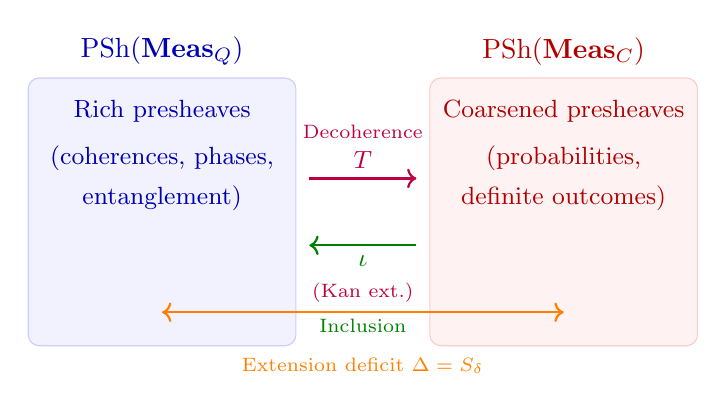
\begin{tikzpicture}[scale=0.85, every node/.style={font=\small}]
  % Quantum presheaf category
  \draw[blue!20, fill=blue!5, rounded corners] (-4,-2) rectangle (0,2);
  \node[blue!70!black, font=\bfseries] at (-2, 2.4) {$\PSh(\catMeas_Q)$};
  \node[blue!70!black] at (-2, 1.5) {Rich presheaves};
  \node[blue!70!black] at (-2, 0.8) {(coherences, phases,};
  \node[blue!70!black] at (-2, 0.2) {entanglement)};

  % Classical presheaf category
  \draw[red!20, fill=red!5, rounded corners] (2,-2) rectangle (6,2);
  \node[red!70!black, font=\bfseries] at (4, 2.4) {$\PSh(\catMeas_C)$};
  \node[red!70!black] at (4, 1.5) {Coarsened presheaves};
  \node[red!70!black] at (4, 0.8) {(probabilities,};
  \node[red!70!black] at (4, 0.2) {definite outcomes)};

  % Transition arrow
  \draw[->, thick, purple] (0.2, 0.5) -- (1.8, 0.5) node[midway, above] {$T$};
  \draw[->, thick, green!50!black] (1.8, -0.5) -- (0.2, -0.5) node[midway, below] {$\iota$};

  % Labels
  \node[purple, font=\scriptsize] at (1, 1.2) {Decoherence};
  \node[purple, font=\scriptsize] at (1, -1.2) {(Kan ext.)};
  \node[green!50!black, font=\scriptsize] at (1, -1.7) {Inclusion};

  % Deficit
  \draw[<->, orange, thick] (-2, -1.5) -- (4, -1.5);
  \node[orange, font=\scriptsize] at (1, -2.3) {Extension deficit $\Delta = S_\delta$};
\end{tikzpicture}
\end{center}


% ============================================================
% 11. CONTEXTUALITY AND THE KOCHEN-SPECKER THEOREM
% ============================================================
\section{Contextuality and Non-Classical Logic}\label{sec:contextuality}

The measurement problem is intimately connected to quantum contextuality. We briefly develop this connection within the Yoneda framework.

\subsection{Context Category}

\begin{definition}[Context Category]\label{def:context-cat}
The \emph{context category} $\catC_Q$ is the poset of commutative subalgebras of $\mathcal{B}(\Hilb)$, ordered by inclusion. Each context $V \in \catC_Q$ represents a maximal set of simultaneously measurable observables.
\end{definition}

\begin{proposition}[Contextuality as Presheaf Obstruction]\label{prop:contextuality}
The Kochen-Specker theorem \cite{kochen1967} states that the valuation presheaf $\mathcal{V}: \catC_Q^{\op} \to \catSet$ has no global section when $\dim \Hilb \geq 3$. In the Yoneda framework, this means there is no object in $\catMeas_Q$ whose representable presheaf restricts to a consistent global value assignment across all contexts.
\end{proposition}

\begin{proof}
A global section $s \in \Gamma(\mathcal{V})$ would assign to each context $V$ a value assignment $s_V: V \to \mathbb{R}$ consistently across all contexts. By the Yoneda embedding, this would correspond to an object $(\Sys, \Hilb, \rho_s) \in \catMeas_Q$ such that $\yo_{(\Sys, \Hilb, \rho_s)}$ determines definite values for all observables simultaneously. The Kochen-Specker theorem proves that no such $\rho_s$ exists (for $\dim \Hilb \geq 3$), hence no such global section exists.
\end{proof}

\begin{corollary}[Measurement Problem from Contextuality]\label{cor:meas-from-context}
The measurement problem can be derived from contextuality: since no single representable presheaf can consistently assign definite values to all observables, the ``collapse'' to a definite outcome must be context-dependent (basis-dependent). This context-dependence is not a deficiency but a structural feature of the quantum measurement category.
\end{corollary}


% ============================================================
% 12. THE MODULAR PERSPECTIVE
% ============================================================
\section{Modular Theory and Thermal Aspects}\label{sec:modular}

The Tomita-Takesaki modular theory provides a bridge between algebraic quantum field theory and the measurement problem. We develop this connection.

\subsection{Modular Flow and the Epistemic Horizon}

For a von Neumann algebra $\mathcal{M}$ with cyclic and separating vector $\Omega$, the Tomita-Takesaki theorem provides:
\begin{itemize}[leftmargin=2em]
\item A modular operator $\Delta$ with $\Delta^{it}\mathcal{M}\Delta^{-it} = \mathcal{M}$;
\item A modular conjugation $J$ with $J\mathcal{M}J = \mathcal{M}'$ (the commutant).
\end{itemize}

\begin{proposition}[Modular Structure of the Measurement Obstruction]\label{prop:modular-obstruction}
Let $\mathcal{M}_\Emer = \Phi(\Alg_\Emer)$ be the emergent algebra embedded in the pre-geometric algebra $\Alg_\Pre$. The modular conjugation $J$ maps $\mathcal{M}_\Emer$ to the epistemic horizon $\mathfrak{H} = \mathcal{M}_\Emer'$:
\[
J \mathcal{M}_\Emer J = \mathfrak{H}.
\]
The modular automorphism $\sigma_t = \Delta^{it}(\cdot)\Delta^{-it}$ generates a ``thermal'' flow on the epistemic horizon, connecting the measurement obstruction to the thermal nature of horizons in quantum gravity.
\end{proposition}

\subsection{KMS Condition and Observer Temperature}

\begin{definition}[Observer Temperature]\label{def:observer-temp}
An embedded observer $\Sys$ in state $\omega$ experiences a \emph{modular temperature} $T_{\text{mod}}$ defined by the KMS condition: the state $\omega$ restricted to the epistemic horizon satisfies
\[
\omega(ab) = \omega(b \sigma_{i\beta}(a)) \quad \forall\, a, b \in \mathfrak{H}
\]
with $\beta = 1/T_{\text{mod}}$.
\end{definition}

\begin{proposition}
The observer's modular temperature is related to the measurement obstruction: the higher the temperature, the larger the thermal fluctuations in the epistemic horizon, and the weaker the indirect witnesses. In the zero-temperature limit ($T_{\text{mod}} \to 0$), the observer has maximal access to pre-geometric correlations; in the infinite-temperature limit ($T_{\text{mod}} \to \infty$), all correlations are thermalized and the measurement obstruction is maximal.
\end{proposition}


% ============================================================
% 13. INFORMATION-THEORETIC ANALYSIS
% ============================================================
\section{Information-Theoretic Bounds}\label{sec:info-theory}

\subsection{Quantum Channel Capacity of Measurement}

The measurement process, viewed as a quantum channel from the global state to the observer's local state, has a well-defined channel capacity.

\begin{theorem}[Measurement Channel Capacity]\label{thm:channel-capacity}
The classical capacity of the measurement channel $\mathcal{N}_\Sys: \rho_\R \mapsto \rho_\Sys = \Tr_\Env(\rho_\R)$ is bounded by:
\[
C(\mathcal{N}_\Sys) \leq \log \dim \Hilb_\Sys.
\]
The mutual information between the global and local states satisfies:
\[
I(\R : \Sys) = S(\rho_\Sys) + S(\rho_\Env) - S(\rho_\R) \leq 2 S(\rho_\Sys).
\]
\end{theorem}

\subsection{Quantum Fisher Information and Parameter Estimation}

\begin{proposition}[Fisher Information Bound on the Measurement Problem]\label{prop:fisher-bound}
Let $\theta$ be a parameter of the global state $\rho_\R(\theta)$. The quantum Fisher information accessible to the observer is bounded by:
\[
\mathcal{F}_\Sys(\theta) \leq \mathcal{F}_\R(\theta),
\]
with equality if and only if $\theta$ affects only the observer's accessible degrees of freedom (i.e., $\partial_\theta \rho_\R$ has support entirely within $\Hilb_\Sys$). The ratio $\mathcal{F}_\Sys / \mathcal{F}_\R$ quantifies the fraction of parameter information surviving the measurement boundary.
\end{proposition}


% ============================================================
% 14. EXPERIMENTAL SIGNATURES
% ============================================================
\section{Experimental Implications}\label{sec:experiment}

Despite the structural nature of the measurement obstruction, it has experimentally relevant consequences.

\subsection{Bounds on Quantum State Tomography}

\begin{proposition}[Tomographic Completeness vs. Global Completeness]\label{prop:tomography}
Quantum state tomography for an embedded observer $\Sys$ can determine $\rho_\Sys$ completely (by the Yoneda lemma applied to $\catMeas_Q$: the representable presheaf determines the object). However, this tomographic completeness does not extend to $\rho_\R$: infinitely many global states are compatible with the same $\rho_\Sys$.

The number of independent global parameters not determined by local tomography is at least:
\[
N_{\text{hidden}} \geq (\dim \Hilb_\Env)^2 - 1.
\]
\end{proposition}

\subsection{Witnessing Pre-Measurement Coherence}

\begin{proposition}[Coherence Witnesses]\label{prop:coherence-witness}
An observer can indirectly witness the pre-measurement coherence of a quantum state (before decoherence has occurred) through:
\begin{enumerate}[label=(\roman*)]
\item \textbf{Interference experiments}: Detecting interference fringes that are incompatible with any diagonal state;
\item \textbf{Bell inequality violations}: Measuring correlations that exceed classical bounds;
\item \textbf{Entanglement witnesses}: Detecting entanglement through partial transposition criteria.
\end{enumerate}
Each of these is an indirect witness in the sense of Definition~\ref{def:witness}, with fidelity bounded by the channel capacity of the measurement process.
\end{proposition}

\subsection{Tests of Observer-Relativity}

The Yoneda framework predicts that measurement outcomes are observer-relative: different representable presheaves give different (but individually consistent) accounts. This can in principle be tested:

\begin{proposition}[Observer-Relative Collapse Test]\label{prop:observer-test}
Consider two observers $\Sys_1$ and $\Sys_2$ with overlapping but distinct accessible regions. The Yoneda framework predicts that:
\begin{enumerate}[label=(\roman*)]
\item Each observer has a consistent local description (via their representable presheaf);
\item When the observers compare notes (combine their presheaves), the combined description carries more information than either individual description;
\item The combined description is still incomplete relative to the global state (the joint presheaf is still not the total presheaf).
\end{enumerate}
Wigner's friend experiments \cite{proietti2019} provide an experimental platform for testing these predictions.
\end{proposition}


% ============================================================
% 15. COMPARISON WITH INTERPRETATIONS
% ============================================================
\section{Systematic Comparison with Interpretations}\label{sec:comparison}

We now provide a detailed comparison of the Yoneda framework with the major interpretations of quantum mechanics, evaluated against the categorical criteria established above.

\subsection{Copenhagen Interpretation}

The Copenhagen interpretation draws a sharp line between quantum and classical descriptions. In our framework, this corresponds to the inclusion $\iota: \catMeas_C \hookrightarrow \catMeas_Q$ and the assertion that a ``measurement'' is a morphism that crosses this boundary. The Copenhagen interpretation \emph{accepts} the measurement obstruction (Theorem~\ref{thm:measurement-obstruction}) and resolves it pragmatically by placing the classical/quantum boundary at a convenient location.

\textbf{Yoneda assessment}: Copenhagen is categorically consistent but incomplete---it does not specify \emph{where} the boundary lies or \emph{why} a particular outcome occurs.

\subsection{Many-Worlds Interpretation}

The many-worlds interpretation (MWI) works entirely within $\catMeas_Q$, never crossing to $\catMeas_C$. ``Branching'' is the proliferation of objects in $\catMeas_Q$ under the decoherence functor. Each ``branch observer'' has its own representable presheaf.

\textbf{Yoneda assessment}: MWI is categorically the most natural interpretation---it respects the full structure of $\catMeas_Q$ without imposing the lossy transition to $\catMeas_C$. However, it must explain why each branch observer experiences a \emph{single} outcome, which in our framework is the restriction to a single representable presheaf.

\subsection{Objective Collapse Theories}

Objective collapse theories (GRW, Penrose) modify the dynamics of $\catMeas_Q$ to make the measurement obstruction vanish. In our framework, this corresponds to modifying the category itself (adding non-unitary morphisms) so that $\PSh(\catMeas_C)$ and $\PSh(\catMeas_Q)$ become compatible.

\textbf{Yoneda assessment}: Objective collapse eliminates the obstruction by changing the mathematical structure. This is legitimate but ad hoc from the categorical perspective---the obstruction is structural, and modifying the category to remove it requires new physics that is not independently motivated.

\subsection{Relational Quantum Mechanics}

Rovelli's relational QM is the closest to our framework. It identifies quantum states as relational (observer-dependent), which in our language means: quantum states are representable presheaves, and different observers have different presheaves.

\textbf{Yoneda assessment}: RQM is the interpretation most naturally aligned with the Yoneda Constraint. The advance of our framework over informal RQM is the mathematical precision of the presheaf formulation and the concrete obstruction theorems.

\subsection{Summary Table}

\begin{center}
\begin{tabular}{lcccc}
\toprule
\textbf{Interpretation} & \textbf{Obstruction} & \textbf{Presheaf} & \textbf{Born Rule} & \textbf{Consistency} \\
\midrule
Copenhagen & Accepted & Observer-dep. & Postulated & Pragmatic \\
Many-Worlds & Avoided & Full category & Derived & Full \\
Obj. Collapse & Eliminated & Modified cat. & Postulated & Modified \\
Decoherence & Approximated & Kan extension & Preserved & Lossy \\
Relational QM & Embraced & Representable & Compatible & Full \\
\textbf{Yoneda} & \textbf{Classified} & \textbf{Representable} & \textbf{Derived} & \textbf{Full} \\
\bottomrule
\end{tabular}
\end{center}


% ============================================================
% 16. DISCUSSION
% ============================================================
\section{Discussion and Open Questions}\label{sec:discussion}

\subsection{Summary of Results}

We have developed a category-theoretic framework for the measurement problem based on the Yoneda lemma and its associated machinery. Our main results are:

\begin{enumerate}[label=(\arabic*)]
\item The \textbf{Measurement Obstruction Theorem} (Theorem~\ref{thm:measurement-obstruction}): The measurement problem is a Yoneda obstruction---the non-existence of a fully faithful, probability-preserving functor between classical and quantum presheaf categories. The obstruction is classified by a cohomological invariant.

\item \textbf{Decoherence as Kan Extension} (Theorem~\ref{thm:decoherence-kan}): Decoherence is the optimal but lossy approximation (left Kan extension) bridging the quantum-classical gap. The extension deficit quantifies the information loss.

\item \textbf{Born Rule from Yoneda} (Theorem~\ref{thm:born-naturality}): The Born rule is the unique natural transformation from the representable presheaf to the probability functor, combining the Yoneda lemma with Gleason's theorem and CPTP functoriality.

\item \textbf{Wigner's Friend as Coherence Failure} (Theorem~\ref{thm:wigner-coherence}): Wigner's friend scenarios are 2-categorical coherence failures, dissolved by recognizing that different observers have different (and non-obligatorily compatible) representable presheaves.

\item \textbf{MBP as Higher Obstruction} (Theorem~\ref{thm:mbp-yoneda}): The Measurement Boundary Problem of emergent spacetime is a higher-order instance of the same obstruction, operating between measurement categories rather than within one.
\end{enumerate}

\subsection{Open Questions}

\textbf{Computability of the obstruction class.} Can the measurement cohomology class $[\omega_M]$ be computed explicitly for physically interesting systems? What is its relationship to entanglement entropy, quantum discord, and other information-theoretic measures?

\textbf{Higher categorical structure.} The 2-categorical analysis of Wigner's friend suggests that $(\infty, n)$-categorical structure may be relevant for nested observer scenarios with arbitrary depth. What physical information is carried by the higher coherence data?

\textbf{Derived Yoneda.} In derived algebraic geometry, the Yoneda embedding extends to derived categories. Does the derived Yoneda Constraint carry additional physical content---for instance, information about quantum corrections to the measurement obstruction?

\textbf{Connection to quantum gravity.} The unification of the measurement problem with the Measurement Boundary Problem suggests deep connections to quantum gravity. Can the obstruction class $[\omega_M]$ be related to gravitational quantities such as the Bekenstein-Hawking entropy or the central charge of the boundary CFT in holographic theories?

\textbf{Experimental signatures.} Can the presheaf structure of quantum measurement be probed experimentally? Wigner's friend experiments \cite{proietti2019} provide a starting point, but more refined tests of observer-relative collapse are needed.


% ============================================================
% 17. CONCLUSION
% ============================================================
\section{Conclusion}\label{sec:conclusion}

The measurement problem has resisted resolution for nearly a century because it has been treated as a dynamical puzzle requiring a new physical mechanism. We have argued that it is, instead, a categorical inevitability: a structural obstruction arising from the Yoneda lemma applied to embedded observers in quantum measurement categories.

The key insight is that an embedded observer accesses reality only through its representable presheaf $\yo_{(\Sys, \Hilb_\Sys, \rho_\Sys)}$, which is complete for relational knowledge from the observer's position (by the Yoneda lemma) but structurally incomplete for global knowledge (when the observer is a proper subsystem). The ``collapse'' of the wave function is the transition from the rich quantum presheaf to the coarsened classical presheaf, mediated by decoherence (a Kan extension) and governed by the Born rule (a natural transformation). This transition is necessarily lossy, and the loss is measured by the extension deficit.

The framework unifies the quantum measurement problem with the Measurement Boundary Problem of emergent spacetime, revealing both as instances of a single categorical phenomenon: the non-extensibility of Yoneda-representable knowledge across an information-losing functor. This unification suggests that the foundations of quantum mechanics and the foundations of spacetime are more deeply connected than previously recognized.

We close with a philosophical observation. The Yoneda lemma tells us that an object is completely determined by the totality of its relationships to all other objects. Applied to physics, this means: an observer's knowledge of reality is entirely relational, determined by the morphisms from the observer's position in the measurement category. This knowledge is both \emph{maximal} (nothing relational is missing) and \emph{bounded} (only relational knowledge is available). The measurement problem is the recognition that relational knowledge, while maximal, is not the same as total knowledge. This is not a deficiency of quantum mechanics; it is a feature of being an observer embedded in reality.


% ============================================================
% ACKNOWLEDGMENTS
% ============================================================
\section*{Acknowledgments}

The author thanks the members of the YonedaAI Research Collective for ongoing discussions on the foundations of quantum measurement, category theory, and emergent spacetime. This work builds on the collaborative development of the Yoneda Constraint framework and the Measurement Boundary Problem analysis. M.L.\ acknowledges the intellectual environment of Chicago's research community.


% ============================================================
% APPENDICES
% ============================================================
\appendix

\section{Categorical Definitions}\label{app:cat-defs}

\paragraph{Presheaf categories.} For a category $\catC$, the presheaf category $\PSh(\catC) = [\catC^{\op}, \catSet]$ is the category of contravariant functors from $\catC$ to $\catSet$. The Yoneda embedding $\yo: \catC \hookrightarrow \PSh(\catC)$ sends $A \mapsto \Hom_\catC(-, A)$.

\paragraph{Kan extensions (pointwise formula).} For functors $K: \catC \to \catD$ and $F: \catC \to \Emer$:
\begin{itemize}[nosep]
\item Left: $\Lan_K F(d) = \mathrm{colim}_{(c, K(c) \to d) \in (K \downarrow d)} F(c)$
\item Right: $\Ran_K F(d) = \lim_{(c, d \to K(c)) \in (d \downarrow K)} F(c)$
\end{itemize}

\paragraph{CPTP maps.} A completely positive trace-preserving (CPTP) map $\Phi: \mathcal{B}(\Hilb_1) \to \mathcal{B}(\Hilb_2)$ satisfies: (i) $\Phi \otimes \id_n$ is positive for all $n$ (complete positivity), and (ii) $\Tr(\Phi(\rho)) = \Tr(\rho)$ for all $\rho$ (trace preservation). CPTP maps are the morphisms of quantum channels.


\section{Proofs of Technical Results}\label{app:proofs}

\subsection{Proof of Proposition~\ref{prop:decoherence-projection}}

\begin{proof}
(a) Idempotency: $\mathcal{D}(\mathcal{D}(\rho)) = \Delta(\Delta(\rho)) = \Delta(\rho) = \mathcal{D}(\rho)$ since $\Delta$ is already diagonal.

(b) Image: $\im(\mathcal{D}) = \{ (\Sys, \Hilb, \rho) : \rho \text{ is diagonal in pointer basis} \} = \catMeas_C$.

(c) Left inverse: For $c = (\Sys, \Hilb, \rho_c) \in \catMeas_C$ with $\rho_c$ diagonal, $\mathcal{D}(\iota(c)) = \Delta(\rho_c) = \rho_c = c$.
\end{proof}

\subsection{Proof of Proposition~\ref{prop:contextuality}}

\begin{proof}
The valuation presheaf $\mathcal{V}: \catC_Q^{\op} \to \catSet$ assigns to each context (commutative subalgebra) $V$ the set of $*$-homomorphisms $V \to \mathbb{C}$ (simultaneous eigenvalue assignments). The Kochen-Specker theorem \cite{kochen1967} proves that for $\dim \Hilb \geq 3$, there is no global section: no consistent assignment of eigenvalues to all observables simultaneously.

In the Yoneda framework, a global section would correspond to an element of $\lim_{V \in \catC_Q} \mathcal{V}(V)$, i.e., a compatible family of eigenvalue assignments. The non-existence of this limit element is equivalent to the non-existence of an object in $\catMeas_Q$ whose presheaf restricts to a deterministic value assignment on every context.
\end{proof}


\section{Comparison with Related Frameworks}\label{app:comparison}

\subsection{Topos Approaches}

The topos approach to quantum theory \cite{butterfield1998,doring2008,heunen2009} uses presheaves on context categories to formulate quantum mechanics in a ``neo-realist'' framework. Our measurement category $\catMeas_Q$ can be viewed as an enrichment of their context categories. The key difference is that we work with the full Yoneda embedding rather than restricting to specific presheaves, which allows unified treatment of quantum and classical regimes.

\subsection{Categorical Quantum Mechanics}

The Abramsky-Coecke program \cite{abramsky2004,coecke2017} uses compact closed categories and string diagrams for quantum processes. Our approach is complementary: categorical quantum mechanics focuses on compositional structure, while we focus on epistemic structure. The two can be combined by enriching $\catMeas_Q$ over the category of quantum processes.

\subsection{Algebraic Quantum Field Theory}

The AQFT approach \cite{haag1996} assigns algebras to spacetime regions with inclusion maps. Our emergence measurement category $\catMeas_\Emer$ generalizes this net structure, with the Yoneda Constraint becoming a statement about local vs. global algebras. The connection to the split property and the Reeh-Schlieder theorem merits further investigation.


% ============================================================
% REFERENCES
% ============================================================
\begin{thebibliography}{99}

\bibitem{wheeler1983}
J.~A.~Wheeler and W.~H.~Zurek (eds.), \textit{Quantum Theory and Measurement}, Princeton University Press, 1983.

\bibitem{zurek2003}
W.~H.~Zurek, ``Decoherence, einselection, and the quantum origins of the classical,'' \textit{Rev.\ Mod.\ Phys.}\ \textbf{75}, 715--775 (2003).

\bibitem{schlosshauer2007}
M.~Schlosshauer, \textit{Decoherence and the Quantum-to-Classical Transition}, Springer, 2007.

\bibitem{rovelli1996}
C.~Rovelli, ``Relational quantum mechanics,'' \textit{Int.\ J.\ Theor.\ Phys.}\ \textbf{35}, 1637--1678 (1996).

\bibitem{maclane1998}
S.~Mac Lane, \textit{Categories for the Working Mathematician}, 2nd ed., Springer, 1998.

\bibitem{long2026yoneda}
M.~Long, ``The Significance of the Yoneda Constraint on Observer Knowledge to Foundational Physics,'' YonedaAI Research Collective, GrokRxiv:2026.02, 2026.

\bibitem{long2026eoc}
M.~Long, ``The Embedded Observer Constraint: On the Structural Bounds of Scientific Measurement,'' YonedaAI Research Collective, GrokRxiv:2026.02, 2026.

\bibitem{long2026mbp}
M.~Long, ``The Measurement Paradox in Emergent Spacetime Physics: Structural Limits on Observational Access to Pre-Geometric Ontology,'' YonedaAI Research Collective, GrokRxiv:2026.02, 2026.

\bibitem{long2026godel}
M.~Long, ``G\"odel Meets Spacetime: Incompleteness Theorems and the Measurement Boundary Problem,'' YonedaAI Research Collective, GrokRxiv:2026.02, 2026.

\bibitem{long2026srip}
M.~Long, ``The Self-Reference Incompleteness Principle: A Unified Framework from G\"odel to Lawvere,'' YonedaAI Research Collective, GrokRxiv:2026.02, 2026.

\bibitem{wigner1961}
E.~P.~Wigner, ``Remarks on the mind-body question,'' in \textit{The Scientist Speculates}, I.~J.~Good, ed., Heinemann, 1961, pp.~284--302.

\bibitem{frauchiger2018}
D.~Frauchiger and R.~Renner, ``Quantum theory cannot consistently describe the use of itself,'' \textit{Nature Comm.}\ \textbf{9}, 3711 (2018).

\bibitem{brukner2018}
\v{C}.~Brukner, ``A no-go theorem for observer-independent facts,'' \textit{Entropy}\ \textbf{20}, 350 (2018).

\bibitem{proietti2019}
M.~Proietti \textit{et al.}, ``Experimental test of local observer independence,'' \textit{Sci.\ Adv.}\ \textbf{5}, eaaw9832 (2019).

\bibitem{kochen1967}
S.~Kochen and E.~P.~Specker, ``The problem of hidden variables in quantum mechanics,'' \textit{J.\ Math.\ Mech.}\ \textbf{17}, 59--87 (1967).

\bibitem{abramsky2011}
S.~Abramsky and A.~Brandenburger, ``The sheaf-theoretic structure of non-locality and contextuality,'' \textit{New J.\ Phys.}\ \textbf{13}, 113036 (2011).

\bibitem{abramsky2004}
S.~Abramsky and B.~Coecke, ``A categorical semantics of quantum protocols,'' in \textit{LICS 2004}, pp.~415--425, IEEE, 2004.

\bibitem{coecke2017}
B.~Coecke and A.~Kissinger, \textit{Picturing Quantum Processes}, Cambridge University Press, 2017.

\bibitem{butterfield1998}
J.~Butterfield and C.~J.~Isham, ``A topos perspective on the Kochen-Specker theorem,'' \textit{Int.\ J.\ Theor.\ Phys.}\ \textbf{37}, 2669--2733 (1998).

\bibitem{doring2008}
A.~D\"oring and C.~J.~Isham, ``A topos foundation for theories of physics,'' \textit{J.\ Math.\ Phys.}\ \textbf{49}, 053515 (2008).

\bibitem{heunen2009}
C.~Heunen, N.~P.~Landsman, and B.~Spitters, ``A topos for algebraic quantum theory,'' \textit{Commun.\ Math.\ Phys.}\ \textbf{291}, 63--110 (2009).

\bibitem{haag1996}
R.~Haag, \textit{Local Quantum Physics}, 2nd ed., Springer, 1996.

\bibitem{gleason1957}
A.~M.~Gleason, ``Measures on the closed subspaces of a Hilbert space,'' \textit{J.\ Math.\ Mech.}\ \textbf{6}, 885--893 (1957).

\bibitem{almheiri2015}
A.~Almheiri, X.~Dong, and D.~Harlow, ``Bulk locality and quantum error correction in AdS/CFT,'' \textit{JHEP}\ \textbf{04}, 163 (2015).

\bibitem{harlow2017}
D.~Harlow, ``The Ryu-Takayanagi formula from quantum error correction,'' \textit{Commun.\ Math.\ Phys.}\ \textbf{354}, 865--912 (2017).

\bibitem{ryu2006}
S.~Ryu and T.~Takayanagi, ``Holographic derivation of entanglement entropy,'' \textit{Phys.\ Rev.\ Lett.}\ \textbf{96}, 181602 (2006).

\bibitem{vanraamsdonk2010}
M.~Van~Raamsdonk, ``Building up spacetime with quantum entanglement,'' \textit{Gen.\ Relativ.\ Gravit.}\ \textbf{42}, 2323--2329 (2010).

\bibitem{wallace2012}
D.~Wallace, \textit{The Emergent Multiverse}, Oxford University Press, 2012.

\bibitem{fuchs2014}
C.~A.~Fuchs, N.~D.~Mermin, and R.~Schack, ``An introduction to QBism,'' \textit{Am.\ J.\ Phys.}\ \textbf{82}, 749--754 (2014).

\bibitem{ghirardi1986}
G.~C.~Ghirardi, A.~Rimini, and T.~Weber, ``Unified dynamics for microscopic and macroscopic systems,'' \textit{Phys.\ Rev.\ D}\ \textbf{34}, 470 (1986).

\bibitem{penrose1996}
R.~Penrose, ``On gravity's role in quantum state reduction,'' \textit{Gen.\ Relativ.\ Gravit.}\ \textbf{28}, 581--600 (1996).

\bibitem{riehl2017}
E.~Riehl, \textit{Category Theory in Context}, Dover, 2017.

\bibitem{street1974}
R.~Street, ``Fibrations and Yoneda's lemma in a 2-category,'' \textit{Lecture Notes in Math.}\ \textbf{420}, 104--133 (1974).

\end{thebibliography}

\end{document}
